% !TEX program = xelatex
\documentclass[12pt, a4paper]{ctexart}

% ==================== 宏包 ====================
\usepackage[margin=2.5cm, headheight=14pt]{geometry}
\usepackage{amsmath, amssymb, amsthm}
\usepackage{graphicx}
\usepackage{booktabs}
\usepackage{multirow}
\usepackage{enumitem}
\usepackage{hyperref}
\usepackage{xcolor}
\usepackage{listings}
\usepackage{tikz}
\usetikzlibrary{shapes.geometric, arrows.meta, positioning, fit, calc}
\usepackage{fancyhdr}
\usepackage{titlesec}
\usepackage{caption}

% ==================== 页面样式 ====================
\pagestyle{fancy}
\fancyhf{}
\fancyhead[L]{\small 数据科学导论}
\fancyhead[R]{\small EdgeThemis: 基于形式化验证的因果推理引擎}
\fancyfoot[C]{\thepage}
\renewcommand{\headrulewidth}{0.4pt}

% ==================== 代码样式 ====================
\lstdefinestyle{rust}{
  language=Java,  % listings 没有原生 Rust，用 Java 近似
  basicstyle=\small\ttfamily,
  keywordstyle=\color{blue}\bfseries,
  commentstyle=\color{gray}\itshape,
  stringstyle=\color{red!70!black},
  numbers=left,
  numberstyle=\tiny\color{gray},
  numbersep=8pt,
  frame=single,
  breaklines=true,
  backgroundcolor=\color{gray!5},
  xleftmargin=2em,
  framexleftmargin=1.5em,
  morekeywords={pub, fn, let, mut, struct, impl, self, Self, return, if, else, while, for, in, match, use, mod, crate, const, type, where, async, await, move},
}

\lstdefinestyle{python}{
  language=Python,
  basicstyle=\small\ttfamily,
  keywordstyle=\color{blue}\bfseries,
  commentstyle=\color{gray}\itshape,
  stringstyle=\color{red!70!black},
  numbers=left,
  numberstyle=\tiny\color{gray},
  numbersep=8pt,
  frame=single,
  breaklines=true,
  backgroundcolor=\color{gray!5},
  xleftmargin=2em,
  framexleftmargin=1.5em,
}

% ==================== 标题样式 ====================
\titleformat{\section}{\Large\bfseries\color{black!80}}{\thesection}{1em}{}
\titleformat{\subsection}{\large\bfseries\color{black!80}}{\thesubsection}{1em}{}
\titleformat{\subsubsection}{\normalsize\bfseries\color{black!80}}{\thesubsubsection}{1em}{}

% ==================== 超链接样式 ====================
\hypersetup{
  colorlinks=true,
  linkcolor=blue!70!black,
  urlcolor=blue!70!black,
  citecolor=blue!70!black,
}

% ==================== 正文开始 ====================
\begin{document}

% ==================== 封面 ====================
\begin{titlepage}
\centering
\vspace*{3cm}

{\Huge\bfseries 数据科学导论\par}
\vspace{1.5cm}

{\LARGE\bfseries EdgeThemis: 基于形式化验证的\\[0.3em]因果推理引擎\par}
\vspace{0.5cm}
{\Large A Causal Reasoning Engine with Formal Verification\par}

\vspace{3cm}

\begin{tabular}{rl}
{\large\bfseries 姓\hfill 名：} & {\large 崔鹏宇} \\[0.8em]
{\large\bfseries 学\hfill 号：} & {\large 2309404018} \\[0.8em]
{\large\bfseries 专\hfill 业：} & {\large 人工智能} \\[0.8em]
{\large\bfseries 日\hfill 期：} & {\large 2026 年 6 月} \\
\end{tabular}

\vfill
\end{titlepage}

% ==================== 摘要 ====================
\newpage
\begin{abstract}
\noindent 大语言模型（LLM）在因果推理任务中存在严重的``拓扑幻觉''问题：生成的因果图可能包含逻辑环路、忽略混淆因子、或产生虚假的因果关联。本文介绍 EdgeThemis——一个专为边缘硬件设计的混合架构因果推理引擎。该系统将形式化数学验证（Rust）无缝嵌入大模型推理循环（Python 状态机），通过三大核心机制保障因果图的逻辑一致性：（1）Kahn 拓扑排序算法检测环路；（2）Bayesian Ball 算法验证 d-分离条件独立性；（3）FMEA（失效模式与影响分析）工业风险评分量化每条因果边的风险等级。系统还引入了自反思纠错闭环，当验证失败时将拦截报告反馈给 LLM 进行自动修正，最多 5 轮熔断。消融实验表明，完整系统（Config C）在 DAG 合法性、d-分离一致性、FMEA 标注和自纠错能力四个维度均显著优于纯 LLM 基线。本系统基于 MSR（2023）关于 LLM 因果推理缺陷的研究和 Reflexion（NeurIPS 2023）的自反思框架，首次将工业 FMEA 方法论与 LLM 因果推理结合，在 8GB VRAM 的 RTX 4060 边缘硬件上实现了工业级的因果推理保障。

\vspace{1em}
\noindent\textbf{关键词：}因果推理；形式化验证；大语言模型；d-分离；FMEA；边缘计算
\end{abstract}

\newpage
\tableofcontents
\newpage

% ==================== 1. 引言 ====================
\section{引言}

\subsection{研究背景}

因果推理是科学发现和工程决策的基石。在医疗诊断、工业故障分析、自动驾驶等领域，准确识别变量之间的因果关系直接关系到决策的正确性和安全性。近年来，大语言模型（Large Language Models, LLM）展现出了从文本中提取因果关系的潜力，但其输出的可靠性面临严峻挑战。

微软研究院（Microsoft Research）在 2024 年 ICLR 发表的工作\cite{msr2024}中，通过构建 Corr2Cause 数据集，残酷地证明了一个事实：\textbf{LLM 本质上是``因果复读机''（Causal Parrots）}——它们只能记住训练语料中的词汇共现模式，一旦面对抽象变量构成的因果问题，表现便退化至随机猜测水平。微调（Fine-tuning）虽然能提升特定数据集上的分数，但面对分布外（OOD）数据时立刻原形毕露。

\subsection{相关工作}

在因果推理增强领域，现有方法可分为以下几个流派：

\begin{enumerate}[label=(\arabic*)]
  \item \textbf{语言反思派}：Reflexion\cite{reflexion2023}（NeurIPS 2023）提出了 Actor$\to$Evaluator$\to$Reflection 的语言强化学习闭环，用自然语言给出强化信号让 LLM 自我纠错。然而，其 Evaluator 是``软性的''——用语言判断对错，无法保证数学绝对确定性。

  \item \textbf{多模型辩论派}：CRAwDAD\cite{crawdad2024}让两个推理大模型互相辩论直至共识。但这种方案需要并发运行多个大参数模型，在 8GB 显存的边缘硬件上毫无落地可能。

  \item \textbf{工具调用派}：Causal Agent\cite{causalagent2024}让 LLM 调用外部 Python 因果库处理表格数据。但若 LLM 在规划链条上产生逻辑幻觉，外部工具再精确也会被带入歧途。
\end{enumerate}

\subsection{本文贡献}

EdgeThemis 走的是第四条路线——\textbf{神经符号学（Neuro-Symbolic）}：用 LLM 做它最擅长的事（从文本中提取因果节点和边），然后直接启动 Rust 底层物理状态机，用编译期的 Kahn 算法和 Bayesian Ball 算法执行 100\% 确定性的数学审判。本文的主要贡献包括：

\begin{enumerate}[label=(\arabic*)]
  \item \textbf{混合架构}：LLM 结构化提取（JSON Schema 强制输出）+ Rust 形式化验证引擎（Kahn 环路检测 + Bayesian Ball d-分离），实现跨语言的确定性因果验证。

  \item \textbf{FMEA 风险量化}：将工业工程中的失效模式与影响分析（FMEA）融入因果图每条边，采用 RPN$=100 \times S + 10 \times O + D$ 公式量化风险等级。

  \item \textbf{自反思纠错闭环}：验证失败时，拦截报告反馈给 LLM 生成器进行定向修复，最多 5 轮熔断，形成``提取--验证--纠错''的自动闭环。
\end{enumerate}

% ==================== 2. 系统架构 ====================
\section{系统架构}

\subsection{整体流水线}

EdgeThemis 采用三层异构架构，如图~\ref{fig:arch}所示。系统流水线为：

\begin{center}
\textbf{Input Text} $\to$ \textbf{Generator (Python)} $\to$ \textbf{Validator (Rust)} $\to$ \textbf{Reflector (Python)} $\to$ \textbf{Output}
\end{center}

\begin{figure}[htbp]
\centering
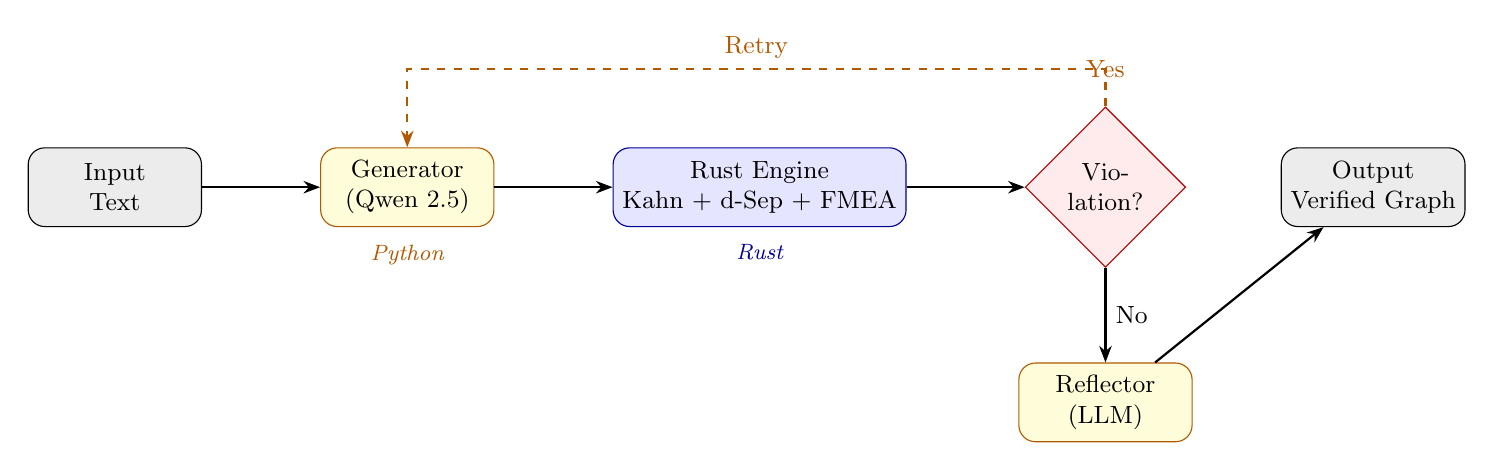
\begin{tikzpicture}[
  node distance=1.2cm and 1.5cm,
  box/.style={rectangle, rounded corners=6pt, draw, minimum width=2.2cm, minimum height=1cm, align=center, font=\small},
  pybox/.style={box, fill=yellow!15, draw=orange!70!black},
  rustbox/.style={box, fill=blue!10, draw=blue!60!black},
  decbox/.style={diamond, draw=red!70!black, fill=red!8, minimum width=1.8cm, minimum height=1.2cm, align=center, font=\small},
  arr/.style={-{Stealth[length=6pt]}, thick},
  darr/.style={arr, dashed, orange!70!black},
]
  % Nodes
  \node[box, fill=gray!15] (input) {Input\\Text};
  \node[pybox, right=of input] (gen) {Generator\\(Qwen 2.5)};
  \node[rustbox, right=of gen] (val) {Rust Engine\\Kahn + d-Sep + FMEA};
  \node[decbox, right=of val] (dec) {Vio-\\lation?};
  \node[pybox, below=1.2cm of dec] (ref) {Reflector\\(LLM)};
  \node[box, fill=gray!15, right=1.2cm of dec] (out) {Output\\Verified Graph};

  % Arrows
  \draw[arr] (input) -- (gen);
  \draw[arr] (gen) -- (val);
  \draw[arr] (val) -- (dec);
  \draw[arr] (dec) -- node[right, font=\small] {No} (ref);
  \draw[arr] (ref) -- (out);
  \draw[darr] (dec) -- node[above, font=\small] {Yes} ++(0,1.5) -| node[above, pos=0.25, font=\small] {Retry} (gen);

  % Labels
  \node[below=0.1cm of gen, font=\footnotesize\itshape, orange!70!black] {Python};
  \node[below=0.1cm of val, font=\footnotesize\itshape, blue!60!black] {Rust};
\end{tikzpicture}
\caption{EdgeThemis 系统架构流水线}
\label{fig:arch}
\end{figure}

\subsection{Generator 节点}

Generator 接收自然语言文本，通过 JSON Schema 约束 LLM 强制输出结构化的 \texttt{CausalEdge} 数据结构。每条边包含五个字段：
\begin{itemize}
  \item \texttt{cause}：原因节点名称
  \item \texttt{effect}：结果节点名称
  \item \texttt{S}（Severity）：严重度，1--10
  \item \texttt{O}（Occurrence）：发生概率，1--10
  \item \texttt{D}（Detection）：检测难度，1--10
\end{itemize}

输出格式由 Pydantic 模型 \texttt{ExtractedGraph} 校验，同时包含 \texttt{reasoning\_process}（Chain-of-Thought 推理链）字段，确保 LLM 先推理再输出结论。

\subsection{Validator 节点}

Validator 是系统的``物理测谎仪''，包含三个并行执行的子模块：
\begin{enumerate}[label=(\arabic*)]
  \item \textbf{Kahn 环路检测}：$O(V+E)$ 拓扑排序，检测因果图中是否存在有向环。
  \item \textbf{Bayesian Ball d-分离}：$O(V^3)$ 方向状态 BFS，全量扫描提取条件独立性断言。
  \item \textbf{FMEA RPN 计算}：对每条因果边独立执行风险评分。
\end{enumerate}

\subsection{Reflector 节点}

Reflector 以``严谨审查员''人格运行，逐一审判 Validator 提取的 d-分离断言。仅在发现结构性逻辑错误时判决 REJECT，触发纠错循环。

% ==================== 3. 核心算法 ====================
\section{核心算法}

\subsection{Kahn 环路检测}

Kahn 算法通过拓扑排序检测有向图中是否存在环路。其核心思想是``剥洋葱''式层层拆解：

\begin{enumerate}
  \item 统计每个节点的入度（被指向的次数）。
  \item 将所有入度为 0 的``自由节点''推入队列。
  \item 依次出队节点，将其所有邻居的入度减 1；若邻居入度变为 0 则入队。
  \item 若成功拆解的节点数等于总节点数，则无环；否则存在环路。
\end{enumerate}

时间复杂度为 $O(V+E)$，其中 $V$ 为节点数，$E$ 为边数。此外，系统在边注入阶段即拦截自环边 $v_i \to v_i$，从源头杜绝无意义的因果回路。

\subsection{Bayesian Ball d-分离算法}

d-分离（directional separation）是因果推理的核心判据，用于判断在给定观测集 $Z$ 的条件下，节点 $X$ 和 $Y$ 是否条件独立。EdgeThemis 采用 Bayesian Ball 算法——一种带方向状态的变种 BFS。

\subsubsection{方向状态}

传统 BFS 只记录 \texttt{visited[node]}，而 Bayesian Ball 记录 \texttt{visited[(node, direction)]}，其中 direction 有两个取值：
\begin{itemize}
  \item \textbf{Up（逆箭头）}：球从当前节点逆着箭头方向移动，寻找父节点（原因）。
  \item \textbf{Down（顺箭头）}：球从当前节点顺着箭头方向移动，寻找子节点（结果）。
\end{itemize}

同一节点在不同方向上可以被多次访问，因为不同方向对应不同的因果结构判定规则。

\subsubsection{四条状态转移规则}

算法的核心是四条状态转移规则，如表~\ref{tab:rules}所示。

\begin{table}[htbp]
\centering
\caption{Bayesian Ball 四条状态转移规则}
\label{tab:rules}
\begin{tabular}{cccccl}
\toprule
\textbf{进入方向} & \textbf{Z 状态} & \textbf{允许 Up?} & \textbf{允许 Down?} & \textbf{对应结构} & \textbf{物理含义} \\
\midrule
Up & 未观测 & \checkmark & \checkmark & Fork $X \leftarrow Z \rightarrow Y$ & 后门大开 \\
Up & 已观测 & $\times$ & $\times$ & Fork $X \leftarrow Z \rightarrow Y$ & 后门关闭 \\
Down & 未观测 & $\times$ & \checkmark & Chain $X \rightarrow Z \rightarrow Y$ & 合法通路 \\
Down & 已观测 & \checkmark & $\times$ & Collider $X \rightarrow Z \leftarrow Y$ & 致命陷阱 \\
\bottomrule
\end{tabular}
\end{table}

\subsubsection{六种判定情况}

三种基本因果结构在观测/未观测两种状态下共产生六种判定情况，如表~\ref{tab:6cases}所示。

\begin{table}[htbp]
\centering
\caption{d-分离六种判定情况}
\label{tab:6cases}
\begin{tabular}{ccccc}
\toprule
\textbf{结构} & \textbf{图示} & \textbf{Z 含 M?} & \textbf{判定} & \textbf{直觉解释} \\
\midrule
Chain & $X \to M \to Y$ & 是 & $X \perp Y$ 阻断 & M 被观测，信息传递截断 \\
Chain & $X \to M \to Y$ & 否 & $X \not\perp Y$ 连通 & 唯一合法因果通路 \\
Fork & $X \leftarrow M \to Y$ & 是 & $X \perp Y$ 阻断 & 共同原因被控制 \\
Fork & $X \leftarrow M \to Y$ & 否 & $X \not\perp Y$ 连通 & 后门大开 \\
Collider & $X \to M \leftarrow Y$ & 是 & $X \not\perp Y$ \textbf{激活} & Explaining away 陷阱 \\
Collider & $X \to M \leftarrow Y$ & 否 & $X \perp Y$ 阻断 & 天然绝缘 \\
\bottomrule
\end{tabular}
\end{table}

其中，Collider（对撞）结构是最反直觉的：观测到中间节点 $M$ 反而\textbf{激活}了 $X$ 和 $Y$ 之间的虚假依赖关系，这称为 \textbf{explaining away} 效应。例如，``业务能力''和``人脉关系''本无关联，但一旦知道某人``已成合伙人''（M 被观测），若发现其业务能力不行，就能推断其靠关系。

\subsection{FMEA 风险评分}

FMEA（Failure Mode and Effects Analysis）是工业工程中广泛使用的风险评估方法。EdgeThemis 将其引入因果推理，每条因果边携带三个维度的评分（S/O/D，取值 1--10），风险优先数 RPN 计算公式为：

\begin{equation}
\text{RPN} = 100 \times S + 10 \times O + D
\label{eq:rpn}
\end{equation}

RPN 的最大值为 $100 \times 10 + 10 \times 10 + 10 = 1110$。系统采用线性加权公式，通过拉大严重度 $S$ 的权重（100 倍），确保高危失效节点在监控中无处遁形。当满足以下任一条件时，系统触发高风险告警：

\begin{itemize}
  \item $\text{RPN} > 500$
  \item $S \geq 9$（致命单点）
\end{itemize}

% ==================== 4. 自反思闭环 ====================
\section{自反思纠错闭环}

自反思闭环是 EdgeThemis 的核心创新之一，其设计借鉴了 Reflexion\cite{reflexion2023} 的 Actor--Evaluator--Reflection 框架，但用 Rust 确定性验证器取代了软性语言评估器。

\subsection{闭环流程}

当 Validator 检测到违规（环路或 d-分离违反）时，拦截报告被反馈给 Generator LLM 进行定向修复：
\begin{enumerate}
  \item \textbf{Round 1}：LLM 提取因果图 $\to$ Rust Kahn 检测到环路 $\to$ 拦截报告反馈。
  \item \textbf{Round 2}：LLM 修正环路 $\to$ Rust Bayesian Ball 发现 d-分离违反 $\to$ 拦截报告反馈。
  \item \textbf{Round 3}：LLM 再次修正 $\to$ 全部验证通过 $\to$ 输出最终因果图。
\end{enumerate}

\subsection{熔断机制}

系统设置 \textbf{5 次拦截上限}（Circuit Breaker）。每次成功生成的图谱被记录为 \texttt{best\_graph}；当验证完全通过时更新。即使触发熔断，系统仍返回历史最佳图谱而非空结果，保障系统的鲁棒性。

\subsection{定向修复}

当 Reflector 判决 REJECT 时，系统将具体的 d-分离断言（最多 10 条）和拒绝理由注入 Generator 的重试 Prompt，并携带上一轮图谱的边列表。Generator 做增量修复而非从头重写，大幅提高纠错效率。

% ==================== 5. 实验与分析 ====================
\section{实验与分析}

\subsection{实验配置}

实验环境配置如表~\ref{tab:config}所示。

\begin{table}[htbp]
\centering
\caption{实验环境配置}
\label{tab:config}
\begin{tabular}{ll}
\toprule
\textbf{项目} & \textbf{配置} \\
\midrule
LLM & Qwen 2.5-3B（Q4 量化） \\
推理框架 & llama-server，OpenAI-compatible API \\
上下文窗口 & 4096 tokens \\
KV Cache & Q8\_0 量化 \\
GPU & RTX 4060（8GB VRAM） \\
测试场景 & 医院感染链路、工业故障传播 \\
\bottomrule
\end{tabular}
\end{table}

\subsection{消融实验}

为验证各模块的增量贡献，设计三组消融对比实验，结果如表~\ref{tab:ablation}所示。

\begin{table}[htbp]
\centering
\caption{消融实验对比}
\label{tab:ablation}
\begin{tabular}{lccc}
\toprule
\textbf{评估指标} & \textbf{Config A: 纯 LLM} & \textbf{Config B: +Schema+Rust} & \textbf{Config C: +Reflection} \\
\midrule
DAG 合法性 & $\times$ 可能含环路 & \checkmark 环路被拦截 & \checkmark 环路被拦截 \\
d-分离一致性 & $\times$ 未验证 & $\triangle$ 检测不修正 & \checkmark 检测+自动修正 \\
FMEA 风险标注 & $\times$ 无 & \checkmark 有 & \checkmark 有 \\
自纠错能力 & $\times$ 无 & $\times$ 无 & \checkmark 最多 5 轮 \\
综合图质量 & 低 & 中 & \textbf{高} \\
\bottomrule
\end{tabular}
\end{table}

消融实验表明：Config A（纯 LLM）可能产生环路，综合质量最低；Config B 加入 Rust 验证后，环路被拦截、FMEA 标注有了，但 d-分离问题只能检测不能修正；Config C（完整 EdgeThemis）在所有维度均表现最优。

\subsection{案例分析}

以医院感染场景为例。Config A 的输出存在 $D \to A$ 的环路，违反 DAG 约束，无 FMEA 标注。经过 Config C 的 3 轮自反思修正后，环路消除，每条边标注了 FMEA RPN 风险值，高风险边（如``败血症患者$\to$死亡''，RPN=1010，S=9）被自动告警。

% ==================== 6. 结论 ====================
\section{结论}

本文介绍了 EdgeThemis——一个基于形式化验证的因果推理引擎。通过将 Rust 图论算子嵌入 LLM 推理循环，系统实现了以下突破：

\begin{enumerate}
  \item 首次将 FMEA 工业风险评估与 LLM 因果推理结合，实现因果边级别的风险量化。
  \item Bayesian Ball d-分离 + Kahn 环路检测实现轻量级形式化验证，$O(V+E)$ 环路检测 + $O(V^3)$ d-分离。
  \item 自反思闭环显著提升因果图逻辑一致性，最多 5 轮自动修正。
\end{enumerate}

已知局限包括：$O(V^3)$ 算法在节点数 $N>50$ 时计算量呈立方级增长；边缘量化模型在多轮重试中可能出现 JSON 语法截断和 FMEA 评分``方差坍塌''。未来计划扩展至更大规模因果图、引入人类反馈机制、并支持时序因果推理。

% ==================== 参考文献 ====================
\newpage
\begin{thebibliography}{9}

\bibitem{msr2024}
J.~Chen et al., ``Can Large Language Models Infer Causation from Correlation?,'' in \textit{Proc. ICLR}, 2024.

\bibitem{reflexion2023}
N.~Shinn et al., ``Reflexion: Language Agents with Verbal Reinforcement Learning,'' in \textit{Proc. NeurIPS}, 2023.

\bibitem{causalflip2025}
CausalFlip: A Benchmark for LLM Causal Judgment Beyond Semantic Matching, \textit{arXiv:2602.20094}, 2025.

\bibitem{crawdad2024}
CRAwDAD: Causal Reasoning Augmentation with Dual-Agent Debate, \textit{arXiv:2511.22854}, 2024.

\bibitem{causalagent2024}
Causal Agent based on Large Language Model, \textit{arXiv:2408.06849}, 2024.

\end{thebibliography}

% ==================== 附录 A：Rust 核心代码 ====================
\newpage
\appendix
\section{附录 A：Rust 核心代码}

\subsection{dag.rs — 紧凑邻接表}

\begin{lstlisting}[style=rust, caption={CompactCausalGraph 结构体定义}]
#[derive(Debug, Clone)]
pub struct CompactCausalGraph {
    pub adjacency_list: Vec<Vec<usize>>,
    pub rev_adjacency_list: Vec<Vec<usize>>,
    pub node_count: usize,
}

impl CompactCausalGraph {
    pub fn new(initial_capacity: usize) -> Self {
        CompactCausalGraph {
            adjacency_list: vec![Vec::new(); initial_capacity],
            rev_adjacency_list: vec![Vec::new(); initial_capacity],
            node_count: 0,
        }
    }

    pub fn add_edge(&mut self, from_id: usize, to_id: usize) {
        self.ensure_capacity(from_id.max(to_id));
        if !self.adjacency_list[from_id].contains(&to_id) {
            self.adjacency_list[from_id].push(to_id);
            self.rev_adjacency_list[to_id].push(from_id);
        }
    }
}
\end{lstlisting}

\subsection{algorithms.rs — Kahn 环路检测（关键片段）}

\begin{lstlisting}[style=rust, caption={Kahn 拓扑排序环路检测}]
pub fn kahn_cycle_detect(graph: &CompactCausalGraph) -> bool {
    let n = graph.node_count;
    if n == 0 { return true; }
    let mut in_degree = vec![0; n];
    for from_node in 0..n {
        if from_node < graph.adjacency_list.len() {
            for &to_node in &graph.adjacency_list[from_node] {
                in_degree[to_node] += 1;
            }
        }
    }
    let mut queue: Vec<usize> = (0..n)
        .filter(|&i| in_degree[i] == 0).collect();
    let mut processed = 0;
    while let Some(node) = queue.pop() {
        processed += 1;
        if node < graph.adjacency_list.len() {
            for &neighbor in &graph.adjacency_list[node] {
                in_degree[neighbor] -= 1;
                if in_degree[neighbor] == 0 {
                    queue.push(neighbor);
                }
            }
        }
    }
    processed == n  // true = 无环, false = 有环
}
\end{lstlisting}

\subsection{algorithms.rs — Bayesian Ball d-分离（关键片段）}

\begin{lstlisting}[style=rust, caption={Bayesian Ball 方向状态 BFS 核心循环}]
pub fn is_d_separated(
    graph: &CompactCausalGraph,
    x: usize, y: usize,
    observed: &HashSet<usize>
) -> bool {
    let rev_adj = graph.rev_adj();
    // 预计算观测节点的祖先（用于 Collider 激活判断）
    let mut ancestors_of_observed = HashSet::new();
    let mut q = VecDeque::new();
    for &obs in observed {
        q.push_back(obs);
        ancestors_of_observed.insert(obs);
    }
    while let Some(node) = q.pop_front() {
        for &parent in &rev_adj[node] {
            if ancestors_of_observed.insert(parent) {
                q.push_back(parent);
            }
        }
    }
    // 贝叶斯球开始滚动
    let mut queue = VecDeque::new();
    let mut visited = HashSet::new();
    queue.push_back((x, false)); // false = Up
    visited.insert((x, false));
    while let Some((curr, is_down)) = queue.pop_front() {
        if curr == y { return false; } // 球到终点 = 未分离
        let is_start = curr == x;
        // Rule 1/2: Up 方向
        if !is_down && (is_start || !observed.contains(&curr)) {
            for &child in &graph.adjacency_list[curr] {
                if visited.insert((child, true)) {
                    queue.push_back((child, true));
                }
            }
        }
        // Rule 4: Down + 已观测 → 允许 Up (Collider 激活)
        else if is_down {
            if is_start || ancestors_of_observed.contains(&curr) {
                for &parent in &rev_adj[curr] {
                    if visited.insert((parent, false)) {
                        queue.push_back((parent, false));
                    }
                }
            }
        }
        // Rule 3: Down + 未观测 → 只允许 Down
        if !is_down && (is_start || !observed.contains(&curr)) {
            for &parent in &rev_adj[curr] {
                if visited.insert((parent, false)) {
                    queue.push_back((parent, false));
                }
            }
        } else if is_down && (is_start || !observed.contains(&curr)) {
            for &child in &graph.adjacency_list[curr] {
                if visited.insert((child, true)) {
                    queue.push_back((child, true));
                }
            }
        }
    }
    true // 球没到 Y = 被 d-分离
}
\end{lstlisting}

\subsection{fmea\_evaluator.rs — FMEA RPN 评分}

\begin{lstlisting}[style=rust, caption={FMEA 风险评分}]
#[pyclass]
pub struct FmeaScore {
    pub s: u32, pub o: u32, pub d: u32,
}

#[pymethods]
impl FmeaScore {
    #[new]
    pub fn new(s: u32, o: u32, d: u32) -> PyResult<Self> {
        if s < 1 || s > 10 || o < 1 || o > 10 || d < 1 || d > 10 {
            return Err(pyo3::exceptions::PyValueError::new_err(
                "S/O/D must be in range 1-10"
            ));
        }
        Ok(FmeaScore { s, o, d })
    }

    pub fn calculate_rpn(&self) -> u32 {
        (100 * self.s) + (10 * self.o) + self.d
    }
}
\end{lstlisting}

% ==================== 附录 B：Python 管线代码 ====================
\newpage
\section{附录 B：Python 管线代码}

\subsection{agent\_state\_machine.py — 数据模型}

\begin{lstlisting}[style=python, caption={Pydantic 数据模型定义}]
from pydantic import BaseModel
from typing import TypedDict, List

class CausalEdge(BaseModel):
    cause: str
    effect: str
    S: int  # Severity (1-10)
    O: int  # Occurrence (1-10)
    D: int  # Detection (1-10)

class ExtractedGraph(BaseModel):
    nodes: List[str]
    edges: List[CausalEdge]
    reasoning_process: str

class ReflectorVerdict(BaseModel):
    verdict: str  # "PASS" or "REJECT"
    reason: str

class CausalAgentState(TypedDict):
    input_text: str
    extracted_graph: dict
    is_safe: bool
    d_separation_claims: List[str]
    rust_interception_report: str
    interception_count: int
\end{lstlisting}

\subsection{nodes.py — Validator 节点（关键片段）}

\begin{lstlisting}[style=python, caption={Validator 节点：FMEA 风险告警逻辑}]
def validate_graph_node(state):
    edges = state["extracted_graph"]["edges"]
    # FMEA RPN 告警
    fmea_alerts = []
    for edge in edges:
        rpn = 100 * edge.S + 10 * edge.O + edge.D
        if rpn > 500:
            fmea_alerts.append(
                f"高危 RPN: {edge.cause}->{edge.effect} ({rpn})"
            )
        if edge.S >= 9:
            fmea_alerts.append(
                f"致命单点: {edge.cause}->{edge.effect} (S={edge.S})"
            )
    # Kahn 环路检测
    topology_safe = rust_engine.kahn_cycle_detect()
    # Bayesian Ball d-分离
    if topology_safe:
        claims = rust_engine.extract_testable_claims()
    return {"is_safe": topology_safe and not claims,
            "d_separation_claims": claims}
\end{lstlisting}

\subsection{app.py — LangGraph 状态机组装（关键片段）}

\begin{lstlisting}[style=python, caption={LangGraph 状态机路由逻辑}]
from langgraph.graph import StateGraph, START, END

def route_after_validate(state):
    if state.get("interception_count", 0) >= 5:
        return END  # 熔断
    if not state.get("is_safe"):
        if state.get("d_separation_claims"):
            return "reflector"
        return "generate"  # 环路 → 直接重试
    return END

def route_after_reflector(state):
    if state.get("interception_count", 0) >= 5:
        return END  # 熔断
    if state.get("verdict") == "REJECT":
        return "generate"
    return END

graph = StateGraph(CausalAgentState)
graph.add_node("generate", generate_graph_node)
graph.add_node("validate", validate_graph_node)
graph.add_node("reflector", reflector_node)
graph.add_edge(START, "generate")
graph.add_edge("generate", "validate")
graph.add_conditional_edges("validate", route_after_validate)
graph.add_conditional_edges("reflector", route_after_reflector)
\end{lstlisting}

\end{document}
